%%
%% CSD Assignment 1 - Final Technical Report
%% Based on the ACM "acmart" manuscript (single-column) style.
%%
\documentclass[manuscript,screen,review]{acmart}
\usepackage{array}
\newcolumntype{L}[1]{>{\raggedright\arraybackslash}p{#1}}

\AtBeginDocument{%
  \providecommand\BibTeX{{Bib\TeX}}}

% \setcopyright{acmlicensed}
% \acmConference[CSD Assignment 1]{Course: Computer Science and Design}{2026}{Your Institute}
% \acmISBN{}

\begin{document}

%% ================= TITLE & AUTHOR BLOCK =================
\title{AI-based Village Pond Planning System}
\subtitle{CSD Assignment 1 -- Final Technical Report}

\author{Roshan Raj}
\authornote{Roll number 12341830. CS559 Computer Systems Design, Monsoon 2026.}
\affiliation{%
  \institution{Indian Institute of Technology Bhilai}
  \city{Durg}
  \state{Chhattisgarh}
  \country{India}}
\email{roshanraj9136@gmail.com}

\renewcommand{\shortauthors}{Raj}

%% ================= ABSTRACT =================
\begin{abstract}
Where a village pond is dug decides how much rain it will ever catch. This report describes
JalDrishti, the web application I built for this assignment. A user draws the land that is
available for digging on a satellite map, and the system returns the best pond site inside that
land, the catchment that drains to it, the water it can collect in an average year, and a pond
sized to hold that water, all drawn on the map. Terrain comes from the Copernicus 30\,m elevation
model for any location in India, or from an uploaded contour map (KML/KMZ). The analysis fills
depressions with Priority-Flood, routes water with D8, accumulates upstream area, traces the
catchment of the chosen outlet, and estimates runoff with the SCS curve number method applied to
ten years of daily ERA5 rainfall. The system runs on the four lab machines (1 CPU and 512\,MiB
each): a Go gateway serves the website, caches results and balances requests over four Python
workers, and PostgreSQL stores saved sites. A 35\,ha parcel is analysed in 42\,ms once its data
is cached; four workers sustain about 10 new analyses per second, 3.9 times one worker, and
repeated requests are answered from the cache at about 900 per second. Against the surveyed
1\,m contour map, the satellite elevation correlates at $r=0.95$ with a 2.5\,m residual error,
and the ERA5 rainfall mean is within 2\,\% of NASA POWER.
\end{abstract}

\keywords{Village Pond Planning, Geospatial Analysis, Rainwater
  Harvesting, Catchment Estimation, Web GIS, REST APIs}

\maketitle

%% =================
\section{Introduction}
\label{sec:intro}
Most villages in central India depend on the monsoon for almost all of their water: at the
project site near Durg, 1{,}238\,mm of the 1{,}386\,mm annual rainfall falls between June and
September. Village ponds (\emph{talabs}) store that water for irrigation, cattle and groundwater
recharge through the dry months, and new ponds are routinely dug under government schemes. A pond
only works if it sits where runoff actually collects and if it is sized to the water that will
reach it.

The goal of this assignment was a web application that recommends such a site. JalDrishti
takes a piece of land selected on a map, analyses the terrain and rainfall around it, and
returns the pond location, its catchment area and the expected water volume, overlaid on the
map. The sections below follow the template: requirements, architecture, methods, implementation,
course themes, results and limitations.

\subsection{Motivation}
Choosing a pond site by eye is hard in this region because the ground is almost flat. The
catchment of the example in Section~\ref{sec:results} has a mean slope of 0.8\,\% and only
8.4\,m of relief over 31\,ha, so the direction water will flow is not visible on the ground or in
imagery. The land that feeds a pond is also rarely the land where the pond is dug: water arrives
from fields and roads upstream that belong to other people. Rainfall records exist, but as
gridded datasets that a panchayat cannot easily query, and the volume a pond will receive depends
on how the rain falls (a few heavy days produce far more runoff than steady drizzle), not only on
the annual total. A tool that does these steps from a map lets a village administrator compare
parcels in seconds and gives a volume figure to plan the excavation budget with.

\subsection{Scope of the Project}
The system (1) accepts any land parcel drawn on the map anywhere in India, using satellite
elevation, or a parcel inside an uploaded contour map; (2) suggests one pond site inside the
parcel and traces its full catchment, including land outside the parcel; (3) estimates rainfall,
runoff and the volume that can be collected in an average year; (4) sizes an excavated pond
(depth, side slope, surface area, storage) within the parcel; (5) overlays all of this on the map
and lets results be saved or downloaded. It does \emph{not} verify land ownership (the user marks
the land that is available), test soil or infiltration on site, model evaporation, seepage or
groundwater recharge, or produce a structural design of the embankment and spillway.

%% =================
\section{Problem Statement and Requirements}
\label{sec:requirements}
Given a land parcel selected by the user, the system must find a suitable pond location, estimate
the catchment area that drains to it and the water that can be collected, and show all three on
the map, quickly and reliably on the four lab machines. Table~\ref{tab:requirements} maps each
functional requirement from the assignment (Phases 2 and 3) to the module that implements it.

\begin{table}[h]
  \caption{Functional requirements and where they are implemented}
  \label{tab:requirements}
  \begin{tabular}{L{4.2cm}L{8.6cm}}
    \toprule
    Requirement & Implemented in \\
    \midrule
    Satellite imagery display & \texttt{frontend/src/components/MapView.jsx} (Esri World Imagery, with terrain and street layers) \\
    Contour map visualization & \texttt{backend/contours.py} (uploaded lines), \texttt{hydrology.contour\_features} (isolines from the DEM) \\
    Select the land area on the map & \texttt{MapView.jsx} drawing tool (outline or rectangle) \\
    Available-land identification & User-drawn parcel; \texttt{planner.select\_site} keeps the pond inside it \\
    Catchment area estimation & \texttt{backend/hydrology.py}, \texttt{planner.dem\_hydrology} \\
    Historical rainfall query & \texttt{backend/rainfall.py} (Open-Meteo ERA5, 2015--2024) \\
    Runoff volume estimation & \texttt{rainfall.scs\_runoff\_mm}, \texttt{planner.build\_result} \\
    Pond depth / storage recommendation & \texttt{planner.size\_pond}, \texttt{planner.pond\_volume} \\
    Combined overlay / results view & \texttt{MapView.jsx} layers, \texttt{Results.jsx} result sheet \\
    Contour upload API (Phase 2) & \texttt{POST /analyzeContour}, \texttt{/findCatchment} in \texttt{backend/main.py} \\
    \bottomrule
  \end{tabular}
\end{table}

\subsection{Non-Functional Requirements}
\begin{itemize}
  \item \textbf{Performance:} a village-sized parcel (up to 1\,km\textsuperscript{2}) is analysed
    in under 1\,s once its elevation tile and rainfall are cached; the page loads in under 2\,s.
  \item \textbf{Scalability:} throughput grows with the number of workers, and every process stays
    inside its container's 1 CPU and 512\,MiB without being killed for memory.
  \item \textbf{Overload behaviour:} no request waits more than 20\,s for a worker; beyond that,
    or when 256 requests are already waiting, the server answers \texttt{503} with
    \texttt{Retry-After} at once instead of timing out.
  \item \textbf{Availability:} a failed worker is removed within 2\,s and its requests are retried
    elsewhere; if the rainfall service or the database is down, analysis still works.
  \item \textbf{Usability:} works in current desktop and mobile browsers, supports the keyboard,
    and states every error with a way to fix it.
  \item \textbf{Security:} all inputs are validated (polygon size and shape, file type, 25\,MB
    upload limit), uploaded XML is parsed without entity expansion, writes are rate-limited, and
    no credentials are stored in the repository.
\end{itemize}

%% =================
\section{System Architecture and High-Level Design}
\label{sec:architecture}
Only one port of the lab machines is reachable from the campus network: 10.1.75.53:3297, which the
lab host forwards to port 3000 on sys1, so everything enters through one gateway
(Figure~\ref{fig:architecture}). The gateway serves the React application, answers repeated
analyses from its cache, and forwards the rest to the worker with the fewest requests in progress.
The worker reads an elevation window from its memory-mapped Copernicus tiles and rainfall from its
cache (or Open-Meteo, once per area), runs the analysis and returns JSON with the map layers, which
the gateway compresses and caches. Saved sites go to PostgreSQL on sys2. Each machine has one CPU
and runs one worker; the sys1 worker runs at a lower priority so the gateway always gets the CPU.

\begin{figure}[h]
  \centering
  
\includegraphics[width=0.8\linewidth]{figures/architecture}
  \caption{High-level system architecture on the four lab machines.}
  \label{fig:architecture}
  \Description{Browsers reach 10.1.75.53:3297, which is forwarded to port 3000 on sys1. A Go
    gateway on sys1 serves the frontend, caches results and balances analysis requests over four
    Python workers on sys1 to sys4. sys2 also runs PostgreSQL. Workers use memory-mapped
    Copernicus elevation tiles and cached Open-Meteo rainfall.}
\end{figure}

\subsection{Technology Stack}
\begin{itemize}
  \item \textbf{Frontend:} React 19 with Vite, Leaflet through react-leaflet, hand-written SVG
    for the pond cross-section, rainfall chart and diagrams.
  \item \textbf{Backend workers:} Python 3.12, FastAPI and Uvicorn, NumPy, SciPy (TIN
    interpolation and smoothing), contourpy (isolines and polygon outlines), defusedxml (KML
    parsing), tifffile and imagecodecs (decoding the elevation tiles).
  \item \textbf{Gateway:} Go 1.27, standard library only.
  \item \textbf{Database:} PostgreSQL 16 through psycopg2.
  \item \textbf{Data:} Copernicus GLO-30 DEM~\cite{copernicusdem} from AWS Open Data;
    Open-Meteo historical archive~\cite{openmeteo} (ERA5~\cite{hersbach2020era5}) for rainfall;
    Nominatim for place search; Esri, OpenStreetMap and OpenTopoMap map tiles.
\end{itemize}
The brief suggests OpenCV; Phase 2 used it for a colour-threshold vegetation estimate that could
not be validated, so it was dropped, and the raster operations (marching squares, smoothing) come
from contourpy and SciPy. The gateway is in Go because it holds many slow connections on one CPU
with little memory.

%% =================
\section{Methodology}
\label{sec:methodology}
Figure~\ref{fig:pipeline} shows the pipeline. Every step works on a regular grid, so the same code
handles satellite and contour-map terrain, and nothing depends on one particular map.

\begin{figure}[h]
  \centering
  
\includegraphics[width=0.9\linewidth]{figures/pipeline}
  \caption{Analysis pipeline from elevation grid to pond size.}
  \label{fig:pipeline}
  \Description{Eight steps: elevation grid, fill pits, D8 flow, accumulate, pond site,
    catchment, water, pond size.}
\end{figure}

\subsection{Terrain and Elevation Analysis}
\textbf{Satellite elevation.} The Copernicus GLO-30 DEM has one height every arc-second
(30.9\,m north--south and 28.8\,m east--west at 21\textdegree N) and is published as
1\textdegree$\times$1\textdegree{} tiles of $3600\times3600$ values. A worker downloads a tile
once, decodes it and stores it as a raw array that it memory-maps, so reading the window around a
parcel is a slice of the page cache with no decoding. Nine tiles covering 20--23\textdegree N,
80--83\textdegree E (Durg, Bhilai, Raipur; 446\,MB) are pre-loaded; any other tile in India is
downloaded on first use. The window around a parcel starts with a margin of
$\min(\max(1.5\,e, 1.2\,\mathrm{km}), 3\,\mathrm{km})$, where $e$ is the parcel's larger side.

\textbf{Contour maps.} A KML or KMZ file is parsed with defusedxml. The height of each line is
taken from an elevation field, the altitude of its coordinates, the number in its name, or its
description, in that order, so the parser does not assume the sample file's layout. Lines are
densified to half a grid cell and a Delaunay (TIN) surface is interpolated in metres onto square
cells sized to about 70{,}000 cells over the map (2.8\,m for the sample), then smoothed by one cell
with a NaN-aware Gaussian filter. (Phase 2 used a $250\times250$ grid, which for this
$3.2\,\mathrm{km}\times164\,\mathrm{m}$ strip meant $13\times0.66$\,m cells that skewed flow
directions.) The map shows the original lines for uploaded maps and marching-squares isolines of
the smoothed DEM for satellite terrain.

\textbf{Checking the DEM against the survey.} I sampled the DEM at all 3{,}689 vertices of the
92 surveyed 1\,m contours. The two agree closely in shape ($r=0.949$), with a constant offset:
the DEM reads 4.3\,m lower on average (RMSE 5.0\,m), and after removing that offset the RMSE is
2.5\,m. A constant offset, likely a difference of vertical reference between the two sources,
does not change flow directions, which depend only on relative heights.

\subsection{Catchment Area Delineation}
\textbf{Filling pits.} Real DEMs contain small hollows that would trap water. Priority-Flood
with $\varepsilon$~\cite{barnes2014priority} starts from the cells on the edge of the data and
always expands the lowest open cell; a neighbour that is not higher is raised to the next
representable value above the current cell. Every cell then has a strictly downhill path to the
edge, and flats get a tiny gradient towards their outlet. A FIFO queue handles raised cells, so
only real rises use the heap.

\textbf{Flow directions.} D8~\cite{ocallaghan1984d8} sends each cell's water to the neighbour with
the steepest drop per metre, using the true east--west spacing at that latitude for diagonal
distances. It is computed for all cells at once with NumPy.

\textbf{Accumulation, site and catchment.} Visiting cells from highest to lowest filled elevation
is a topological order of the flow graph, so adding each cell's area to its receiver gives the
upstream area of every cell in one pass. The pond site is the cell inside the parcel with the
largest upstream area, ignoring cells on the edge of the data, with ties broken by lower ground.
The catchment is found in the reverse order: a cell belongs to it if its receiver does. If the
catchment touches the edge of the window, the margin is multiplied by 2.2 and the analysis is
repeated, up to 200{,}000 cells; if it still touches, the result is flagged as a lower bound. For
$N$ cells the cost is $O(N\log N)$ for the fill and the sort and $O(N)$ for the rest.

\textbf{Assumptions.} D8 sends all water from a cell in one direction; the DEM is a surface model
that includes trees and buildings; and features smaller than a cell, such as field bunds, are
invisible to it.

\subsection{Rainfall Data Integration}
Rainfall comes from the Open-Meteo historical archive~\cite{openmeteo}, which serves the ERA5
reanalysis~\cite{hersbach2020era5}: daily totals for the ten complete years 2015--2024 at the pond
site, cached per 0.1\textdegree{} cell in memory and on disk. From the series the system reports
the mean annual and monsoon (June--September) rainfall, the wettest day and a per-year table. If
the service cannot be reached, a regional normal of 1{,}150\,mm with a runoff coefficient of 0.25
is used and the result says so.

Runoff uses the SCS curve number method~\cite{scs1972neh4} on every rain day $P$ (mm):
$S = 25400/\mathit{CN} - 254$, $I_a = 0.2S$, and $Q = (P-I_a)^2/(P-I_a+S)$ for $P>I_a$. The curve
number is adjusted each day for antecedent moisture: if the previous five days brought less than
35.6\,mm (growing season) the soil is treated as dry, above 53.3\,mm as wet, using
$\mathit{CN}_\mathrm{I}$ and $\mathit{CN}_\mathrm{III}$ from~\cite{chow1988applied}. This matters
because ERA5 spreads heavy storms over several days; without the adjustment the runoff
coefficient for $\mathit{CN}=80$ was 0.12, with it 0.19. Yearly runoff depth is averaged over the
ten years and multiplied by the catchment area.

The pond is an excavated basin with 1.5:1 side slopes and the chosen depth (3\,m by default). Its
top area is solved so that the frustum volume $V=\tfrac{d}{3}(A_t+A_b+\sqrt{A_tA_b})$ holds the
yearly runoff, but it may not exceed 60\,\% of the parcel or 5\,ha. Its footprint is grown from the
site over the lowest ground in the parcel, with a penalty of 1\,m per 40\,m of distance to keep it
compact. The water collected is $\min(\text{runoff}, V)$.

\textbf{Cross-check.} For the example site, NASA POWER~\cite{nasapower} gives a 2015--2024 mean
of 1{,}364\,mm per year against 1{,}386\,mm from ERA5, a 1.6\,\% difference. Individual years
differ more (yearly correlation 0.64, mean absolute difference 159\,mm), which is why the system
uses the ten-year average rather than any single year.

%% =================
\section{Implementation}
\label{sec:implementation}

\subsection{Backend and API Design}
The workers expose a REST API (Table~\ref{tab:api}), documented with OpenAPI at \texttt{/docs}.
All geometry is GeoJSON with longitude before latitude. There is no login, because the tool is
meant to be open to anyone on the campus network; changes to saved sites are rate-limited per
client at the gateway. Invalid input returns \texttt{400} (wrong file type) or \texttt{422}
(unusable polygon or contour map) with a message saying what to fix. Failures of external
services are handled where they occur: the rainfall fallback above, a \texttt{502} with a clear
message if an elevation tile cannot be downloaded, and a \texttt{503} from the database layer that
affects only saved sites. A worker that is busy answers \texttt{503} with an
\texttt{X-Worker-Busy} header, and the gateway retries the request on another worker.

\begin{table}[h]
  \caption{Main API endpoints}
  \label{tab:api}
  \begin{tabular}{L{5.6cm}L{7.2cm}}
    \toprule
    Method and path & Purpose \\
    \midrule
    \texttt{POST /api/analyze} & Parcel (GeoJSON) and design parameters $\rightarrow$ analysis on satellite terrain \\
    \texttt{POST /api/analyze/contour} & Contour map upload (or sample) and optional parcel $\rightarrow$ analysis \\
    \texttt{POST /analyzeContour}, \texttt{/findCatchment} & Phase 2 contract: field \texttt{contour\_map}; Phase 2 keys plus the full analysis \\
    \texttt{GET /api/sample}, \texttt{/api/sample/contour\_map} & Analysis of the sample map; the sample KML itself \\
    \texttt{GET /api/rainfall}, \texttt{/api/coverage} & Rainfall and runoff at a point; pre-loaded elevation tiles \\
    \texttt{GET|POST|DELETE /api/sites} & Saved sites (PostgreSQL) \\
    \texttt{GET /api/health}, \texttt{/gateway/status} & Worker health; gateway, cache and worker metrics \\
    \bottomrule
  \end{tabular}
\end{table}

\subsection{Frontend and Visualization}
The interface (Figure~\ref{fig:ui}) is a map with a panel of four steps: choose the terrain data,
draw the land (outline or rectangle, with a live area in hectares and acres), set pond depth, land
cover and largest pond, and run the analysis. Results are map layers that can be toggled in the
legend: the parcel (dashed yellow), the pond footprint (dark blue) with a label giving the yearly
volume, the catchment (light blue), flow paths and contours. The result sheet starts with the three
required outputs, then a to-scale cross-section of the pond filled to the yearly runoff, ten years
of rainfall and runoff, and notes. Results can be saved or downloaded as GeoJSON, and a status page
shows live metrics. If all workers are busy, the page retries after \texttt{Retry-After} with
random jitter.

\begin{figure}[h]
  \centering
  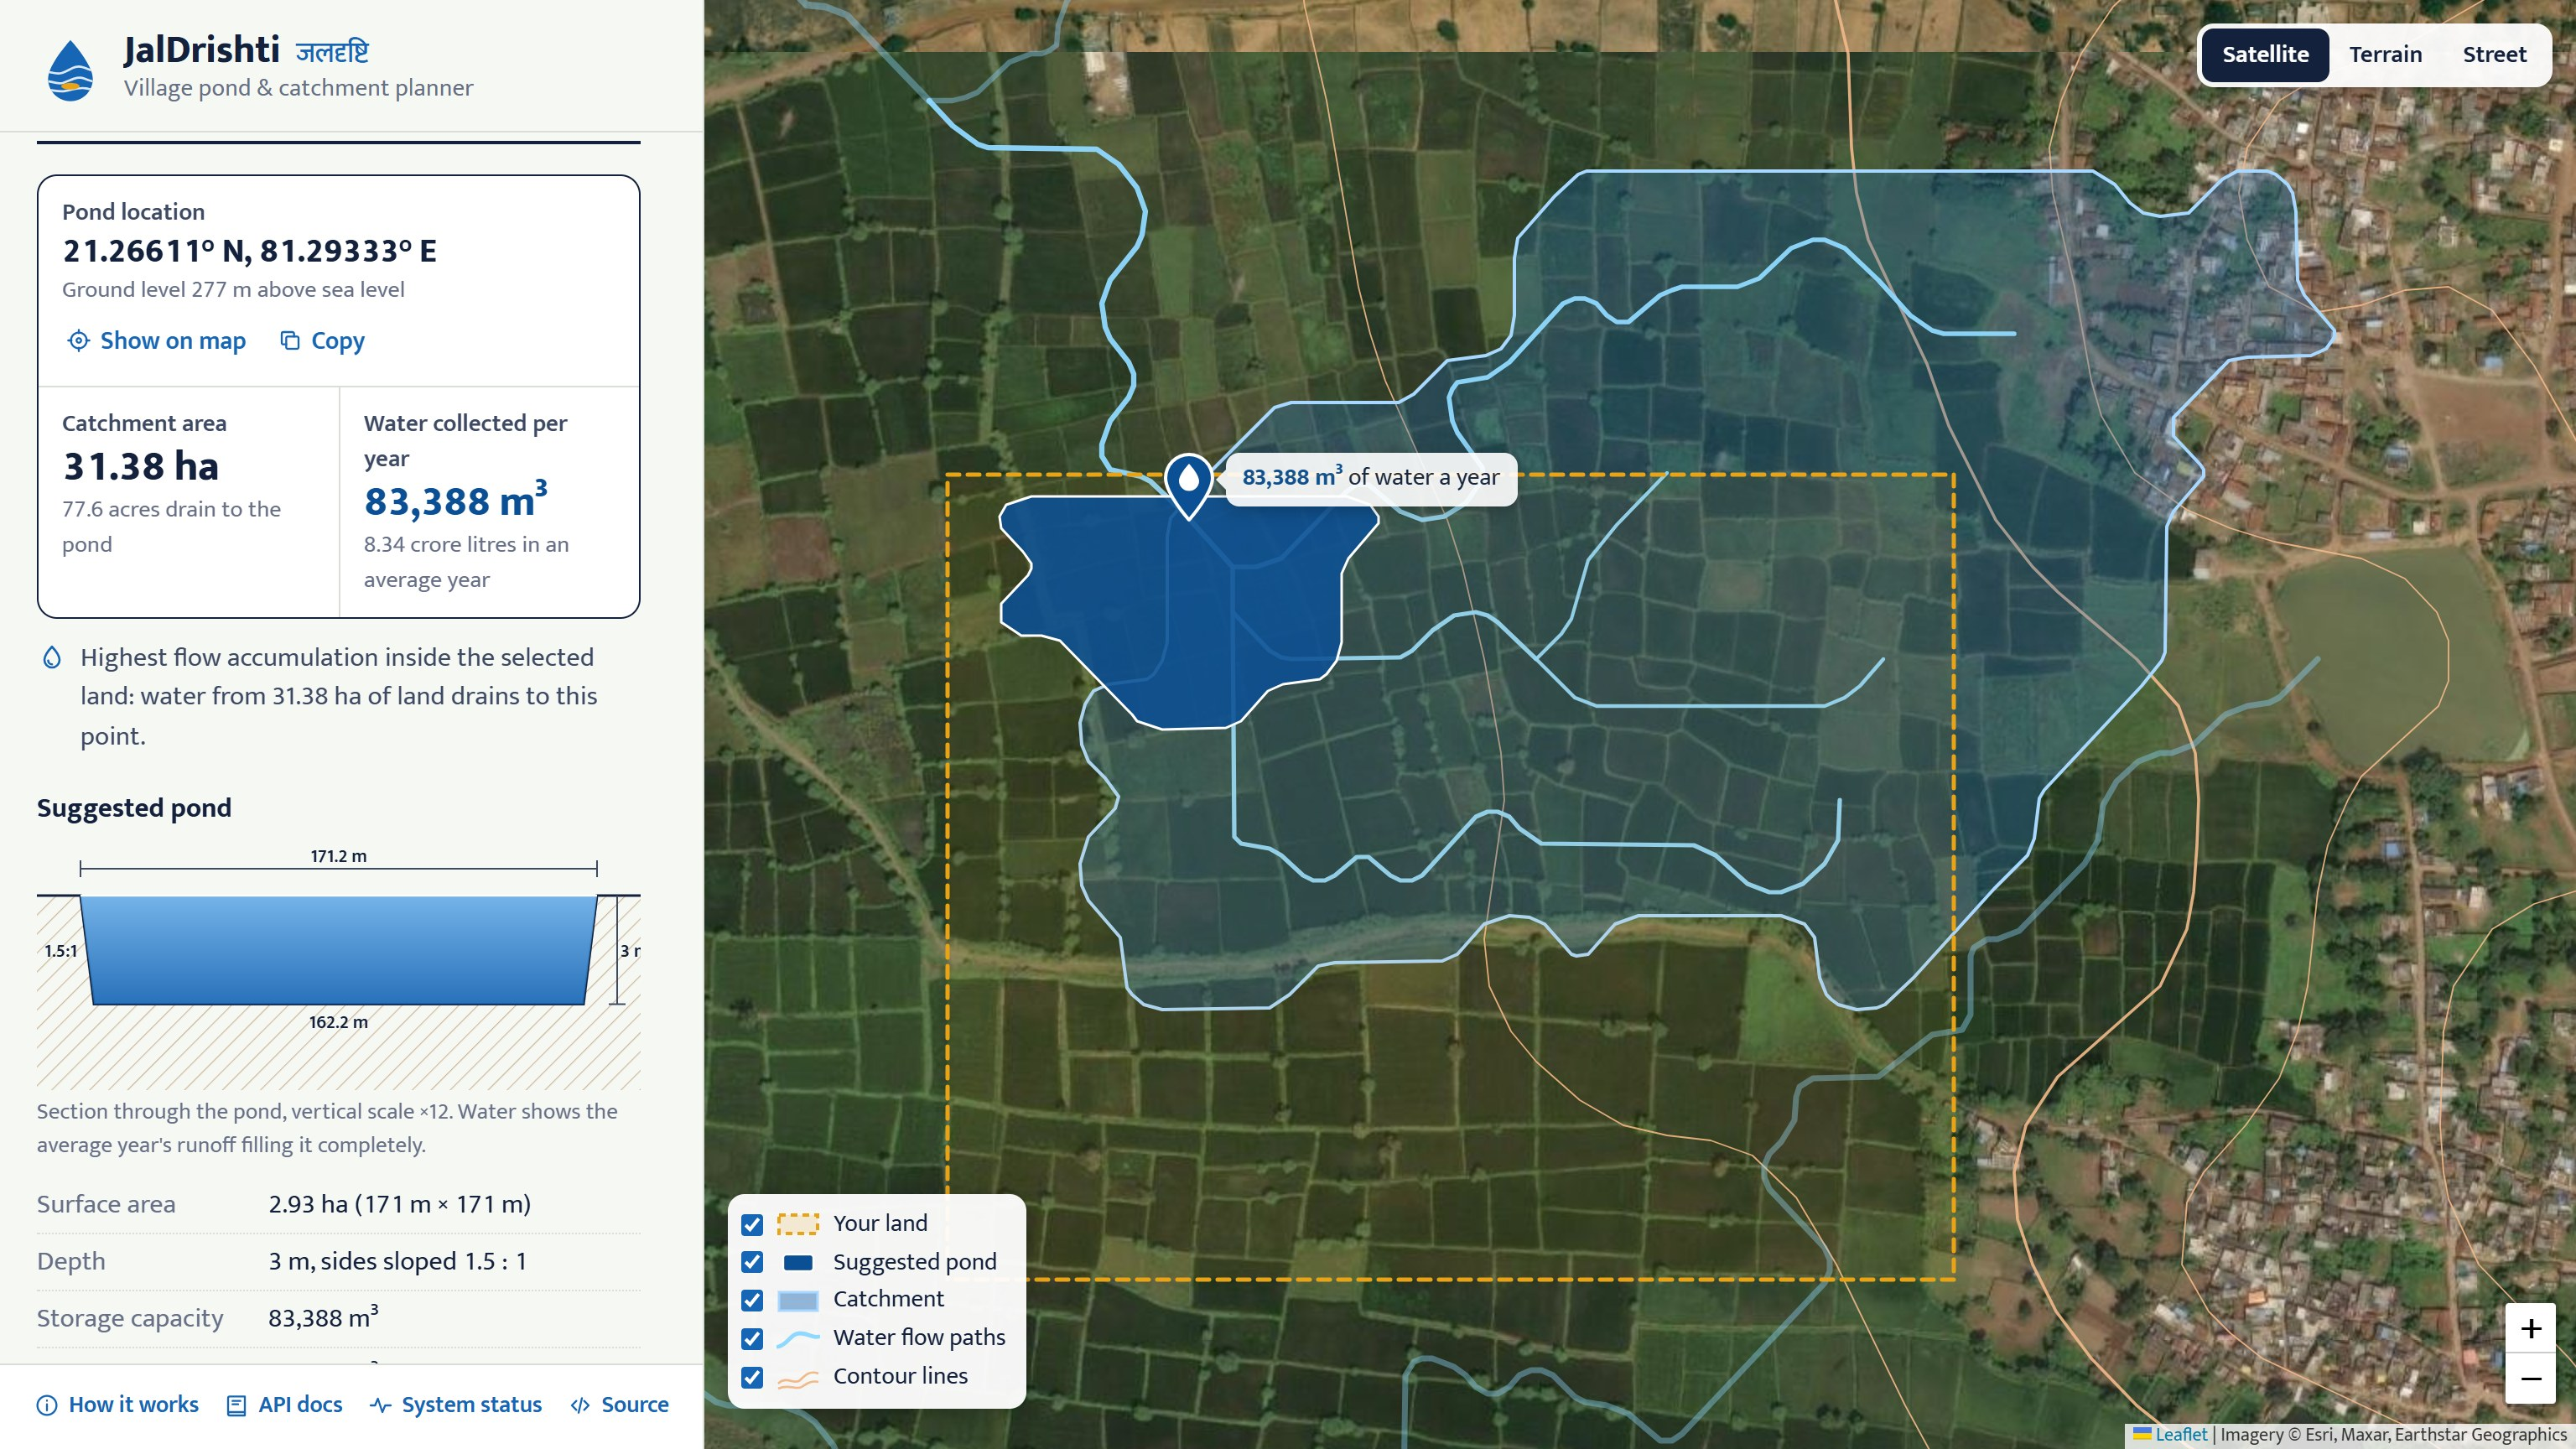
\includegraphics[width=0.8\linewidth]{figures/ui}
  \caption{Application interface showing the results overlay.}
  \label{fig:ui}
  \Description{Left: the result sheet with pond location 21.26611 N, 81.29333 E, catchment area
    31.38 ha, water collected 83,388 cubic metres per year, and a pond cross-section. Right: a
    satellite map with the selected land as a dashed yellow rectangle, the pond footprint in dark
    blue, the catchment in light blue extending beyond the land, flow paths and a legend.}
\end{figure}

\subsection{Database and Storage}
Saved sites live in one PostgreSQL table, \texttt{pond.sites}, created by the first worker that
needs it under an advisory lock. Each row holds the name, pond coordinates, the parcel polygon as
\texttt{jsonb}, and the areas and volumes. The table is capped at 500 rows and read in id order, so
the primary key is the only index needed. Everything else is a cache: elevation tiles as
memory-mapped arrays on each worker's disk, rainfall as one JSON file per 0.1\textdegree{} cell,
the flow model of recently used contour maps in memory keyed by the file's SHA-256 (so drawing a
second parcel on the same map skips the fill and accumulation), and analysis responses in the
gateway (96\,MB of gzip, least recently used, six-hour lifetime).

%% =================
\section{CSD Themes and Topics Applied in the Project}
\label{sec:csd-themes}
Table~\ref{tab:csd-themes} maps the course themes to the parts of the system where they appear.

\begin{table*}[t]
  \caption{Mapping of core CSD themes/topics to their use in this project}
  \label{tab:csd-themes}
  \footnotesize
  \begin{tabular}{L{2.6cm}L{5.0cm}L{6.3cm}}
    \toprule
    CSD Theme/Topic & Where used in the project & Justification / design rationale \\
    \midrule
    API Design (REST) & \texttt{/api/analyze}, \texttt{/api/analyze/contour}, Phase 2 routes, OpenAPI at \texttt{/docs} & Stateless JSON requests can go to any worker and be cached by their content; Phase 2 routes kept so earlier clients still work \\
    Load Balancing & Go gateway: least in-flight worker, health check every 2\,s, retry on another worker & Analyses vary from 40\,ms to over 1\,s, so round-robin would queue short requests behind long ones \\
    Caching & Gateway response cache with single-flight; rainfall per 0.1\textdegree{} cell; DEM page cache; contour flow models & Removes repeated computation and external calls; 63 of 64 identical concurrent requests shared one computation \\
    Database Indexing / Query Optimization & Primary key on \texttt{pond.sites}; tiles read by slicing a memory map & At 500 rows an extra index costs more than it saves; the real query cost is in the elevation data, which needs no decoding \\
    Concurrency / Asynchronous Processing & Async FastAPI with a thread pool, one analysis at a time per worker; goroutines in the gateway & Health checks stay responsive while a worker computes; the CPU-bound step is not run in parallel on one CPU \\
    Microservices vs. Monolith & One analysis service replicated four times behind a gateway, plus a database & Splitting the pipeline into services would add network hops without separate scaling needs \\
    Design Patterns & Gateway (reverse proxy), Strategy for terrain sources, single-flight, cache-aside, fallback & Satellite and contour terrain both produce the same grid, so one pipeline serves both \\
    Authentication / Authorization & None for analysis; writes rate-limited per client & A public planning tool on the campus network; abuse risk is limited to saved-site spam \\
    Containerization / Deployment & Four lab containers; \texttt{bootstrap\_host.sh}, \texttt{pondctl.sh}, rolling \texttt{deploy.sh} & No sudo, systemd or cron on the hosts; restart loops in tmux, and workers restarted one at a time so the site stays up \\
    Error Handling and Resilience & Busy \texttt{503} with retry, rainfall fallback, worker removal on failure, client retry with jitter & The system degrades gracefully instead of timing out \\
    Algorithms and Complexity & Priority-Flood, D8, topological accumulation: $O(N\log N)$ & Correct on flats and pits, where a simple slope heuristic fails \\
    Testing Strategy & Unit and API tests, load tests (Section~\ref{sec:testing}) & Synthetic terrain has known answers; load tests check the non-functional targets \\
    Version Control / CI-CD & GitHub; Actions runs tests, \texttt{go vet} and the frontend build on each push & Deployment pulls the same commit on every host \\
    \bottomrule
  \end{tabular}
\end{table*}

Three decisions mattered most. \textbf{Admission control instead of unbounded queueing.} Each
machine has one CPU and an analysis takes about 0.4\,s on average, so a worker can finish about
2.5 per second. By Little's law~\cite{harcholbalter2013}, anything beyond that only adds waiting
time. The gateway therefore lets each worker hold two requests (one running, one waiting), keeps
at most 256 others in a queue for at most 20\,s, and answers the rest with \texttt{503} at once.
Under 300 concurrent requests this kept throughput at capacity with no crashes, instead of every
request timing out. \textbf{Caching with single-flight.} Many users look at the same village, and
identical concurrent requests are collapsed into one computation before the cache is even filled.
\textbf{Memory as the binding limit.} Each container has 512\,MiB, so tiles are memory-mapped
rather than loaded, BLAS is limited to one thread, and workers return freed memory to the system
after each analysis; together this brought worker memory under load from about 230\,MB to about
150\,MB.

%% =================
\section{Results and Evaluation}
\label{sec:results}
The example parcel is a 35.6\,ha rectangle of farmland near Khapri village, Durg district, the
same one shown in the demo video. Table~\ref{tab:example} lists the results, and
Figure~\ref{fig:ui} shows them on the map. Water from 31.4\,ha drains to the north-west corner of
the parcel, much of it from outside the parcel. The pond there is limited by runoff: a 2.93\,ha,
3\,m deep pond holds the full 83{,}388\,m\textsuperscript{3} of an average year.

\begin{table}[h]
  \caption{Results for the example parcel near Khapri, Durg}
  \label{tab:example}
  \begin{tabular}{L{5.2cm}L{7.6cm}}
    \toprule
    Quantity & Value \\
    \midrule
    Selected land & 35.6\,ha (88.0 acres) \\
    Pond location & 21.26611\textdegree N, 81.29333\textdegree E, ground level 277.0\,m \\
    Catchment area & 31.38\,ha (77.6 acres); mean slope 0.8\,\%, relief 8.4\,m \\
    Rainfall (2015--2024 mean) & 1{,}386\,mm per year, 1{,}238\,mm in June--September \\
    Runoff (CN 80, farmland) & 266\,mm per year, coefficient 0.19 \\
    Runoff reaching the pond & 83{,}388\,m\textsuperscript{3} per year \\
    Pond & 2.93\,ha, 171\,m $\times$ 171\,m at the top, 3\,m deep, sides 1.5:1 \\
    Storage capacity / water collected & 83{,}388\,m\textsuperscript{3} per year (8.3 crore litres) \\
    \bottomrule
  \end{tabular}
\end{table}

The sample contour map (Figure~\ref{fig:results}) is a strip 3.2\,km long and 164\,m wide. Its
surface is a $61\times1176$ grid of 2.8\,m cells. The pond goes at 21.26351\textdegree N,
81.28324\textdegree E (267.9\,m), with a catchment of 14.16\,ha and 37{,}622\,m\textsuperscript{3}
of runoff a year. Because the strip is so narrow, the catchment reaches its edge and the result
says the true catchment may be larger. Phase 2 reported 6.97\,ha and 14{,}801\,m\textsuperscript{3}
for this map; the difference comes from pit filling (Phase 2 routed water into DEM noise), square
cells instead of $13\times0.66$\,m cells, and measured rainfall of 1{,}386\,mm instead of a fixed
850\,mm. For larger parcels the single-pond limit applies: for a 1\,km\textsuperscript{2} parcel
the catchment is 107\,ha and a 5\,ha pond collects 144{,}044 of the 291{,}928\,m\textsuperscript{3}
of runoff, and the result suggests a chain of ponds for the rest.

\begin{figure}[h]
  \centering
  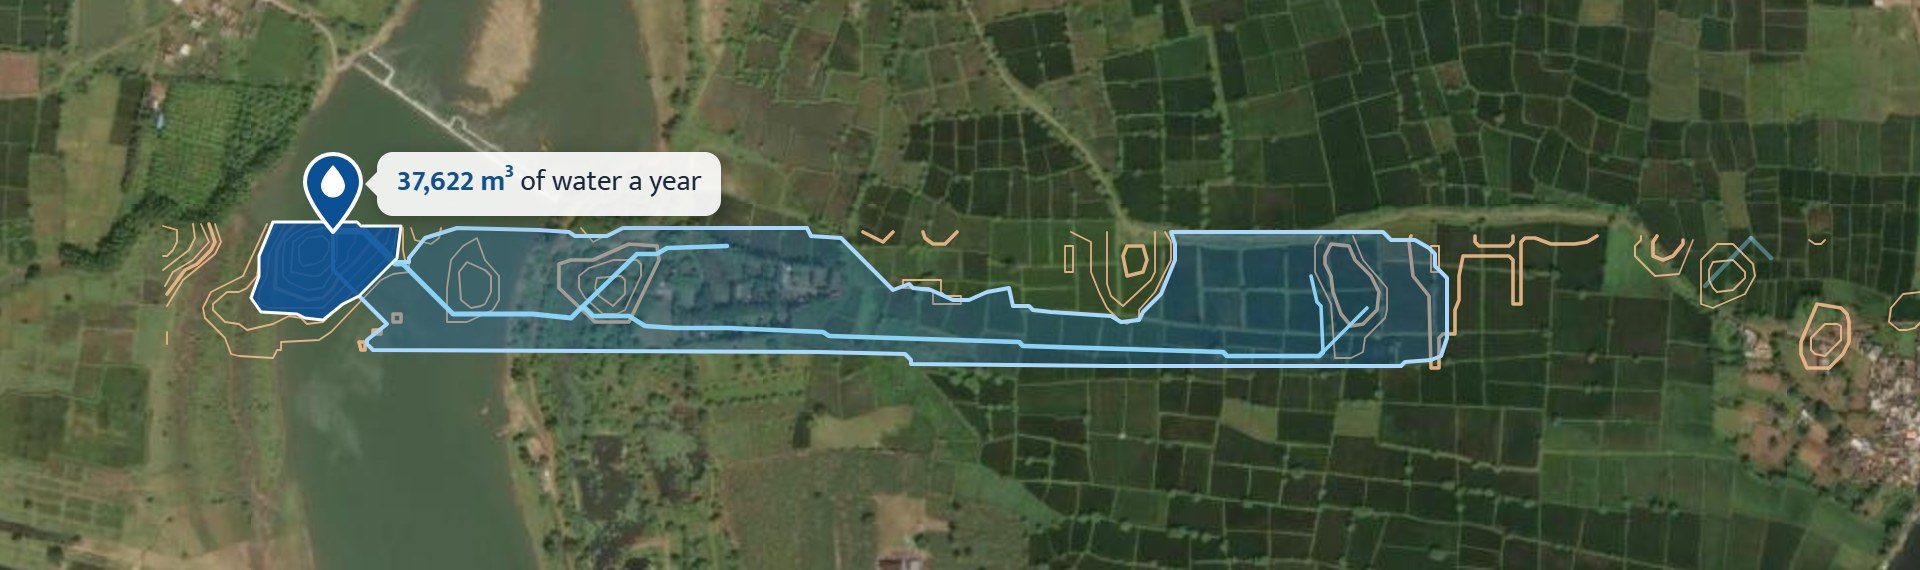
\includegraphics[width=0.9\linewidth]{figures/contour_result}
  \caption{Result for the sample contour map: contour lines, the pond at the west end and the
  catchment along the strip.}
  \label{fig:results}
  \Description{A satellite map of a narrow strip beside a river with orange contour lines, a dark
    blue pond at its west end labelled 37,622 cubic metres a year, and a light blue catchment along
    the strip.}
\end{figure}

\subsection{Performance}
Table~\ref{tab:timings} gives measured times on one worker, as medians of five runs once the
elevation tile and rainfall are cached. For the 4\,km\textsuperscript{2} parcel the window grew
once to fit a 760\,ha catchment; of its 705\,ms, the fill took 278\,ms, flow directions and
accumulation 105\,ms, the catchment 29\,ms, and building the map layers 114\,ms.

\begin{table}[h]
  \caption{Response times for key operations (one worker)}
  \label{tab:timings}
  \begin{tabular}{L{7.4cm}L{5.4cm}}
    \toprule
    Operation & Time \\
    \midrule
    Rainfall for a new 0.1\textdegree{} cell (Open-Meteo) / cached & 1{,}274\,ms / 0.04\,ms \\
    Sample contour map, first upload / same map again & 464\,ms / 47\,ms \\
    Analysis, 12\,ha parcel (8{,}910 cells) & 37\,ms \\
    Analysis, 35.6\,ha example parcel (10{,}573 cells) & 42\,ms \\
    Analysis, 1\,km\textsuperscript{2} parcel (18{,}612 cells) & 65\,ms \\
    Analysis, 4\,km\textsuperscript{2} parcel (195{,}534 cells) & 705\,ms \\
    \bottomrule
  \end{tabular}
\end{table}

Load was generated from a laptop on the campus network against the public address, each request
a different 400\,m $\times$ 300\,m parcel unless stated (Table~\ref{tab:load}). Four workers give
3.9 times the throughput of one, since the work is CPU-bound and shares nothing. At 300 concurrent
requests the excess got an immediate \texttt{503}, and memory stayed near 150\,MB per worker and
60\,MB for the gateway, with no process killed.

\begin{table}[h]
  \caption{Load tests against the public address}
  \label{tab:load}
  \small
  \begin{tabular}{lrrrrr}
    \toprule
    Scenario & Workers & Concurrent & Throughput (/s) & Success & p50 \\
    \midrule
    Unique parcels & 1 & 8 & 2.5 & 100\,\% & 2.9\,s \\
    Unique parcels & 4 & 8 & 9.8 & 100\,\% & 0.61\,s \\
    Unique parcels & 4 & 16 & 8.5--9.5 & 100\,\% & 1.4\,s \\
    Same parcel (cache) & 4 & 64 & 912 & 100\,\% & 60\,ms \\
    80\,\% popular, 20\,\% new & 4 & 32 & 39 & 100\,\% & 33\,ms \\
    Overload, unique & 4 & 300 & 10.3 & 37\,\% (rest \texttt{503}) & 10.6\,s \\
    \bottomrule
  \end{tabular}
\end{table}

\subsection{Testing}
\label{sec:testing}
Fourteen automated tests run on every push through GitHub Actions, with \texttt{go vet} and the
frontend lint and build. Engine tests use synthetic terrain with known answers: accumulation must
peak at a valley's outlet, a pit must be filled so every cell drains, a pond must sit on the lowest
valley cell inside its parcel, and a ridge must keep a pond from collecting the next valley's water.
API tests cover the Phase 2 contract on the sample map, wrong file types, KML without elevations,
XML entity attacks, and tiny or self-crossing polygons. Load tests check the performance targets,
and every deployment ends with a smoke test of all public links.

%% =================
\section{Discussion and Limitations}
\label{sec:discussion}
Pit filling removed the scattered sinks that made the Phase 2 result depend on noise, one pipeline
serves both terrain sources, and the gateway made four small machines behave as one service;
watching memory rather than CPU is what kept it stable. The main limits are in the data. The DEM is a surface model at 30\,m, so trees and
buildings raise it and field bunds, which steer water between fields, are invisible; results on
very flat land are therefore approximate. The sample contour map is too narrow to contain a whole
catchment. ERA5 smooths the heaviest storms, and the curve numbers are standard values, not
calibrated for local soils. The pond sizing ignores evaporation and seepage, which are large in
this climate, and sizing to one average year's runoff is a planning rule, not a design. D8 also
sends all water from a cell one way, which concentrates flow on flats. Finally, the land must still
be checked against revenue records. Natural next steps are multiple-flow routing, IMD gridded
rainfall, soil-based curve numbers, and ranking several candidate sites instead of one.

%% =================
\section{AI Tool Usage Declaration}
\label{sec:ai-usage}
Claude (Anthropic), used through the Claude Code command-line tool, assisted with this assignment:
writing and refactoring code for the backend, gateway and frontend, debugging, writing the
deployment and load-test scripts, drafting the README, the diagrams and this report, and producing
the demo video, whose narration uses a synthetic Microsoft Edge text-to-speech voice. I directed
the work from the assignment brief, decided what the system should do and how it would run on the
lab machines, and take responsibility for all submitted code and text.

\bibliographystyle{ACM-Reference-Format}
\bibliography{report}

%% =================
\appendix

\section{Source Code and Repository}
{\raggedright
Repository: \url{https://github.com/roshanraj9136/village_pond_planner}\\
Live application: \url{http://10.1.75.53:3297} (API documentation at \texttt{/docs}, live metrics
at \texttt{/status})\\
Demo video: \url{https://youtu.be/Q3VEN3Mh6os}\\
Folders: \texttt{backend/} (FastAPI worker: \texttt{hydrology.py}, \texttt{planner.py},
\texttt{dem.py}, \texttt{contours.py}, \texttt{rainfall.py}, \texttt{sites.py}, \texttt{main.py},
\texttt{tests/}); \texttt{gateway/} (Go gateway); \texttt{frontend/} (React and Leaflet);
\texttt{deploy/} (host setup, service control, rolling deployment, load test); \texttt{docs/},
\texttt{report/} and \texttt{sample\_data/}. The README explains how to run and deploy it.\par}

\end{document}
\endinput
